\documentclass[11pt,a4paper]{article}
\usepackage[margin=2cm]{geometry}
\usepackage{graphicx}
\usepackage{adjustbox}
\usepackage{float}
\usepackage{booktabs}
\usepackage{xcolor}
\usepackage{listings}
\usepackage{tikz}
\usepackage[colorlinks=true,linkcolor=blue]{hyperref}

\lstset{basicstyle=\ttfamily\footnotesize,breaklines=true,frame=single,
        backgroundcolor=\color{gray!8},columns=fullflexible,keepspaces=true}
\setlength{\parindent}{0pt}
\setlength{\parskip}{0.5em}

\title{Computer Networks Course Project\\[2pt]
\large Phase 1: Build and Observe the Network -- Team 1}
\author{Vikrant (Mac 1) \quad Asad (Mac 2) \quad Mayank (Mac 3) \quad Prashant (Mac 4)}
\date{}

\begin{document}
\maketitle

% ============================================================
\section{Team Introduction and Setup Flow}

We built a small private service platform on four MacBooks connected to the same Wi-Fi
(network 10.7.0.0/19, gateway 10.7.0.1). A client types a private name,
\texttt{app.team1.test}; our own DNS server resolves it; the client opens an HTTPS
connection to our nginx edge; and nginx forwards the request to one of two backend servers.

\begin{table}[H]
\centering
\begin{tabular}{llllll}
\toprule
Machine & Person & Role & Service / port & IPv4 & Interface \\
\midrule
Mac 1 & Vikrant  & Private DNS server        & dnsmasq, UDP 53   & 10.7.13.235 & en0 \\
Mac 2 & Asad     & Edge proxy + load balancer & nginx, TCP 8443   & 10.7.17.39  & en0 \\
Mac 3 & Mayank   & Backend A + client        & Python REST, 3001 & 10.7.5.187  & en0 \\
Mac 4 & Prashant & Backend B + client        & Python REST, 3002 & 10.7.15.184 & en0 \\
\bottomrule
\end{tabular}
\end{table}

\begin{figure}[H]
\centering
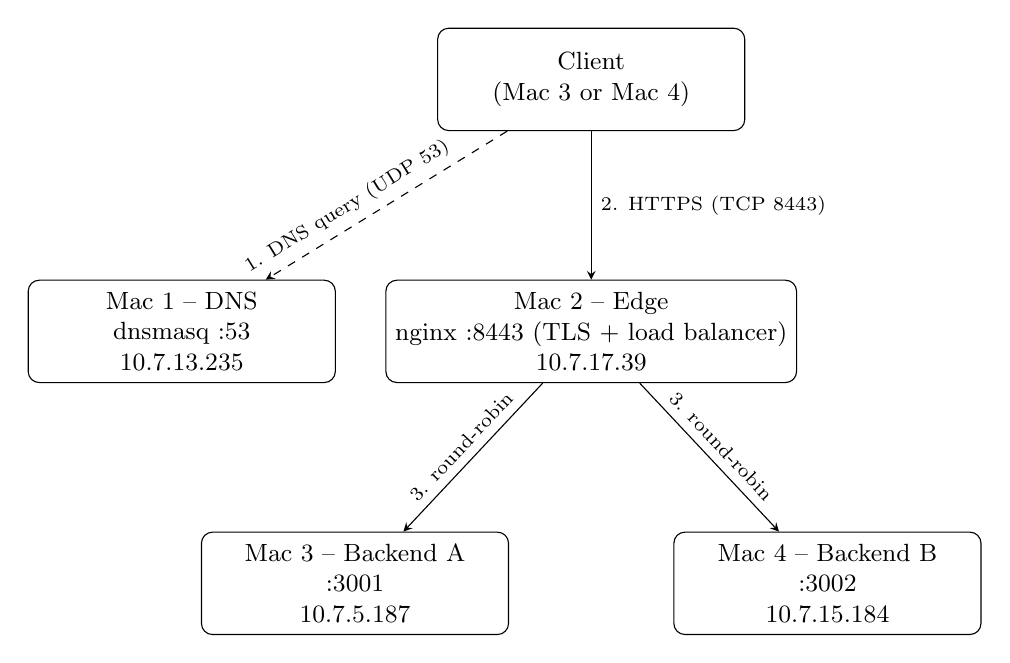
\begin{tikzpicture}[box/.style={draw,rounded corners,minimum width=3.9cm,minimum height=1.3cm,align=center,font=\small},
                    >=stealth]
\node[box] (client) at (0,3.2) {Client\\(Mac 3 or Mac 4)};
\node[box] (dns)    at (-5.2,0) {Mac 1 -- DNS\\dnsmasq :53\\10.7.13.235};
\node[box] (edge)   at (0,0) {Mac 2 -- Edge\\nginx :8443 (TLS + load balancer)\\10.7.17.39};
\node[box] (a)      at (-3,-3.2) {Mac 3 -- Backend A\\:3001\\10.7.5.187};
\node[box] (b)      at (3,-3.2) {Mac 4 -- Backend B\\:3002\\10.7.15.184};
\draw[->,dashed] (client) -- node[above,sloped,pos=0.62,font=\scriptsize]{1. DNS query (UDP 53)} (dns);
\draw[->] (client) -- node[right,font=\scriptsize]{2. HTTPS (TCP 8443)} (edge);
\draw[->] (edge) -- node[above,sloped,font=\scriptsize]{3. round-robin} (a);
\draw[->] (edge) -- node[above,sloped,font=\scriptsize]{3. round-robin} (b);
\end{tikzpicture}
\caption{Network topology and request flow.}
\end{figure}

\subsection*{Setup flow (Task A and Task B)}
\begin{enumerate}
\item All four Macs joined the same Wi-Fi. We recorded each Mac's interface, IPv4 address, mask
      (255.255.224.0 = /19), gateway and MAC address (full table in \texttt{docs/ARCHITECTURE.md}).
\item We checked reachability by pinging every pair of machines: 4 packets, 0\% packet loss each.
\item Mac 1 runs dnsmasq with records for \texttt{app.team1.test} and \texttt{api.team1.test} pointing
      to the edge (Mac 2). Mac 3 and Mac 4 use Mac 1 as their DNS resolver.
\end{enumerate}

\begin{figure}[H]
\centering
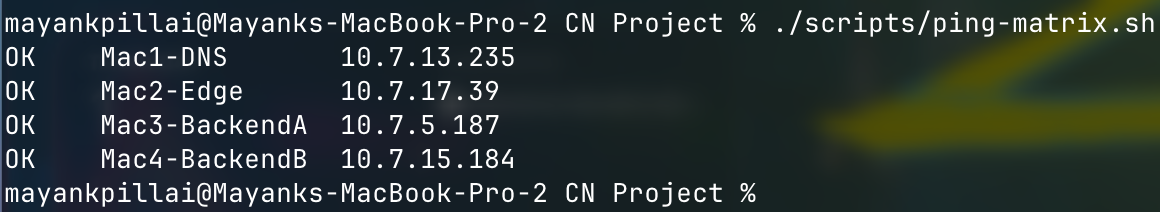
\includegraphics[width=0.8\linewidth]{../evidence/taskA-lan/taskA-mac3-pingmatrix.png}
\caption{Task A: Mac 3 can reach all four machines (all OK).}
\end{figure}

\begin{figure}[H]
\centering
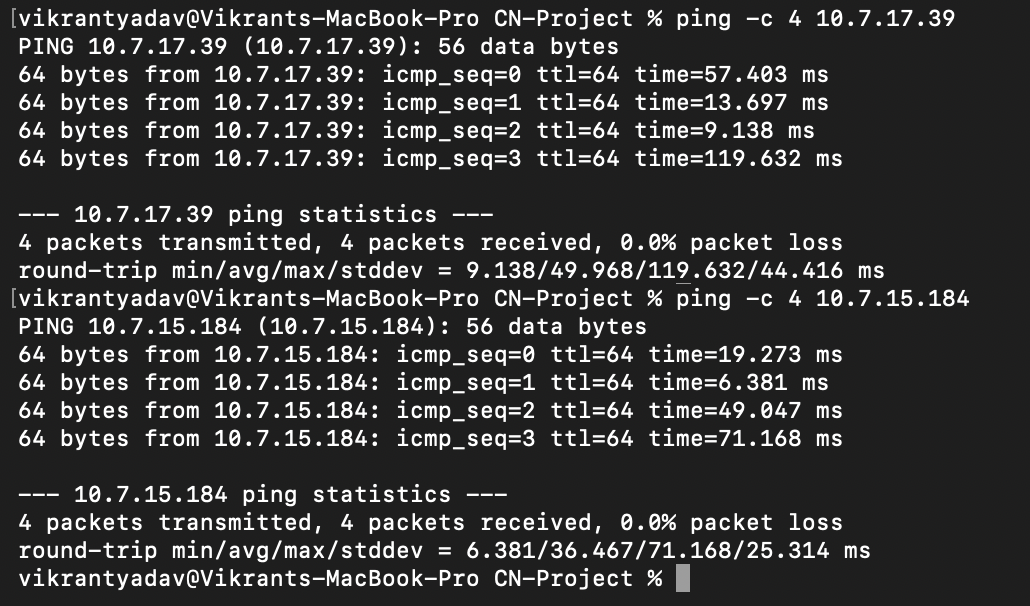
\includegraphics[width=0.7\linewidth]{../evidence/taskA-lan/taskA-mac1-ping.png}
\caption{Task A: Mac 1 to Mac 2 and Mac 4, 4 packets each, 0\% loss.}
\end{figure}

\begin{figure}[H]
\centering
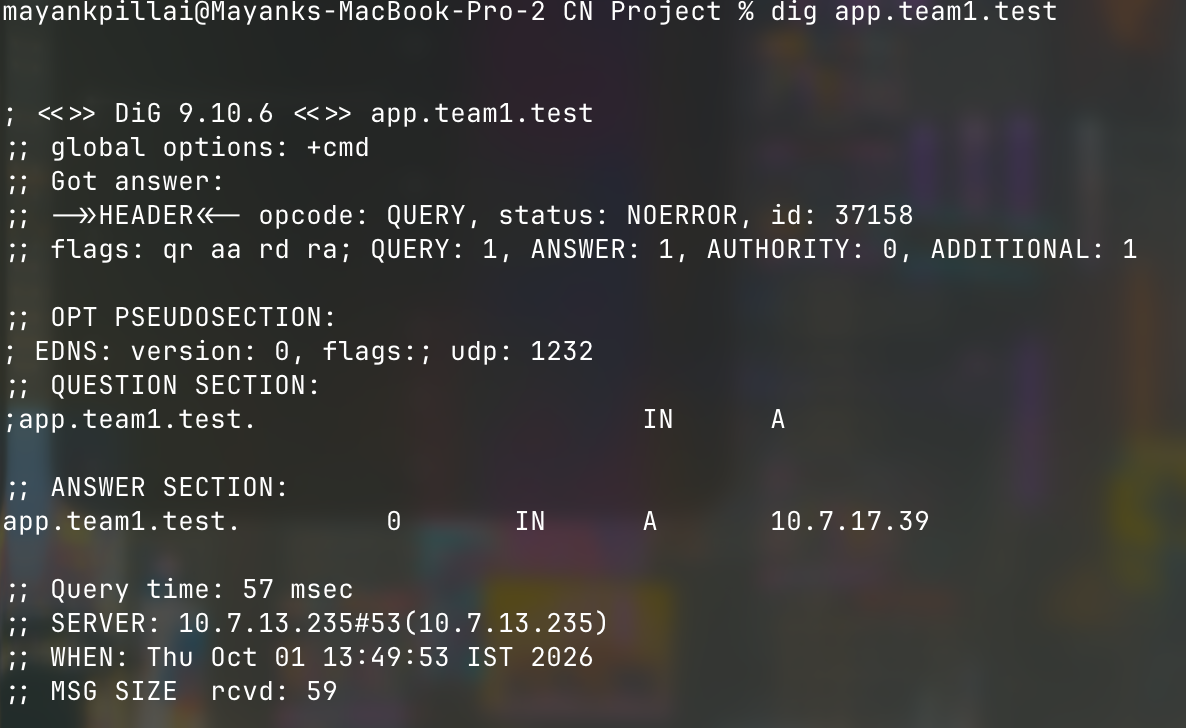
\includegraphics[width=0.7\linewidth]{../evidence/taskB-dns/taskB-mac3-dig.png}
\caption{Task B: \texttt{dig app.team1.test} from a client (Mac 3). The answer is the edge IP
10.7.17.39 and the SERVER line is our DNS server 10.7.13.235.}
\end{figure}

% ============================================================
\newpage
\section{How the Configuration Works}

\subsection{DNS server (Mac 1, dnsmasq)}
dnsmasq listens on Mac 1's LAN address (not only 127.0.0.1), so other machines can use it, and
answers for our two names with the edge's IP.
\lstinputlisting{../config/dnsmasq.conf}

In the capture below, the client (10.7.5.187, UDP port 58206) asks the DNS server
(10.7.13.235, port 53) for \texttt{app.team1.test}; the answer is 10.7.17.39 with TTL 0.
\begin{figure}[H]
\centering
\adjustbox{width=\linewidth,trim={0 {.82\height} 0 0},clip}{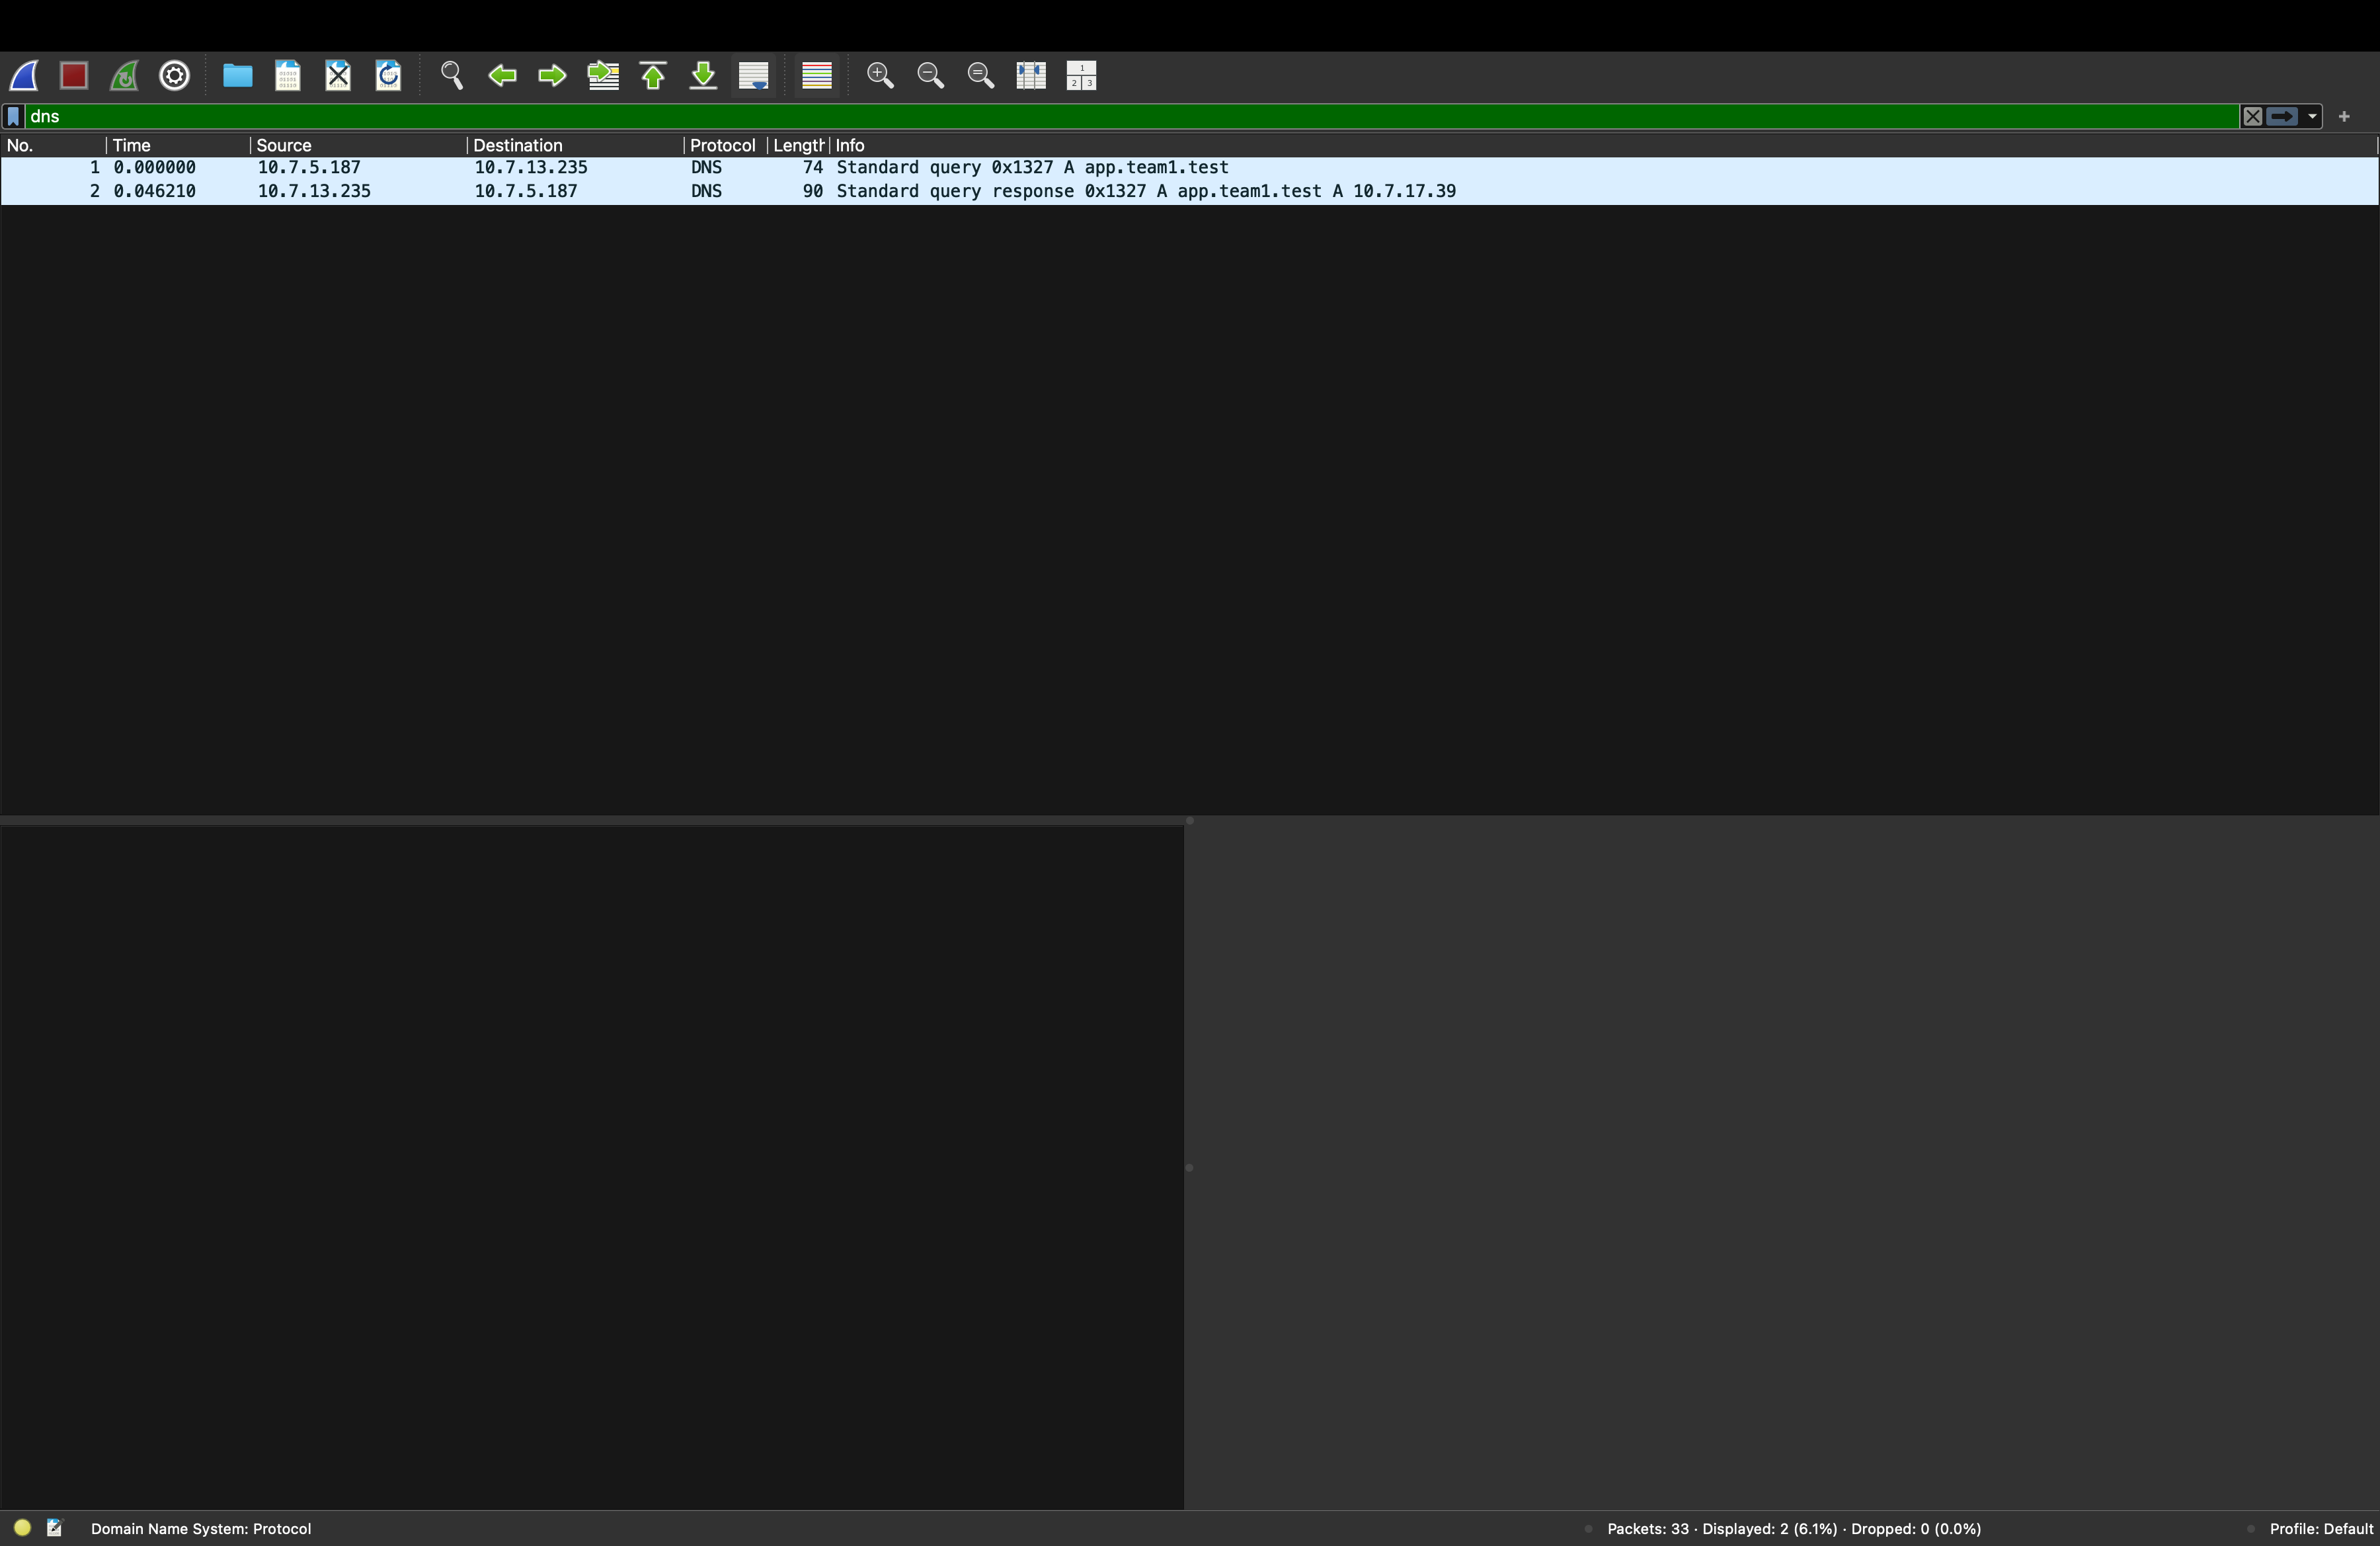
\includegraphics{../evidence/taskG-packet-analysis/dns-flow.png}}
\caption{Wireshark filter \texttt{dns}: query (frame 1) and response (frame 2).}
\end{figure}

\subsection{Backends (Mac 3 and Mac 4)}
Each backend is a small Python HTTP server that listens on all interfaces (0.0.0.0), on port 3001
(A) or 3002 (B). It answers \texttt{GET /} and \texttt{GET /api/status}, and every response carries
an \texttt{X-Backend: A} (or \texttt{B}) header and \texttt{Cache-Control: max-age=60}.
The code is in \texttt{backend/backend\_a.py} and \texttt{backend/backend\_b.py}.

\subsection{nginx edge: TLS termination and load balancing (Mac 2)}
nginx is the single entry point. It terminates TLS on port 8443 with a certificate for
\texttt{app.team1.test} and \texttt{api.team1.test} created with mkcert (approved by our faculty), and
forwards requests round-robin to the two backends, so clients never learn the backend IPs.
\lstinputlisting{../config/nginx.conf}

\begin{figure}[H]
\centering
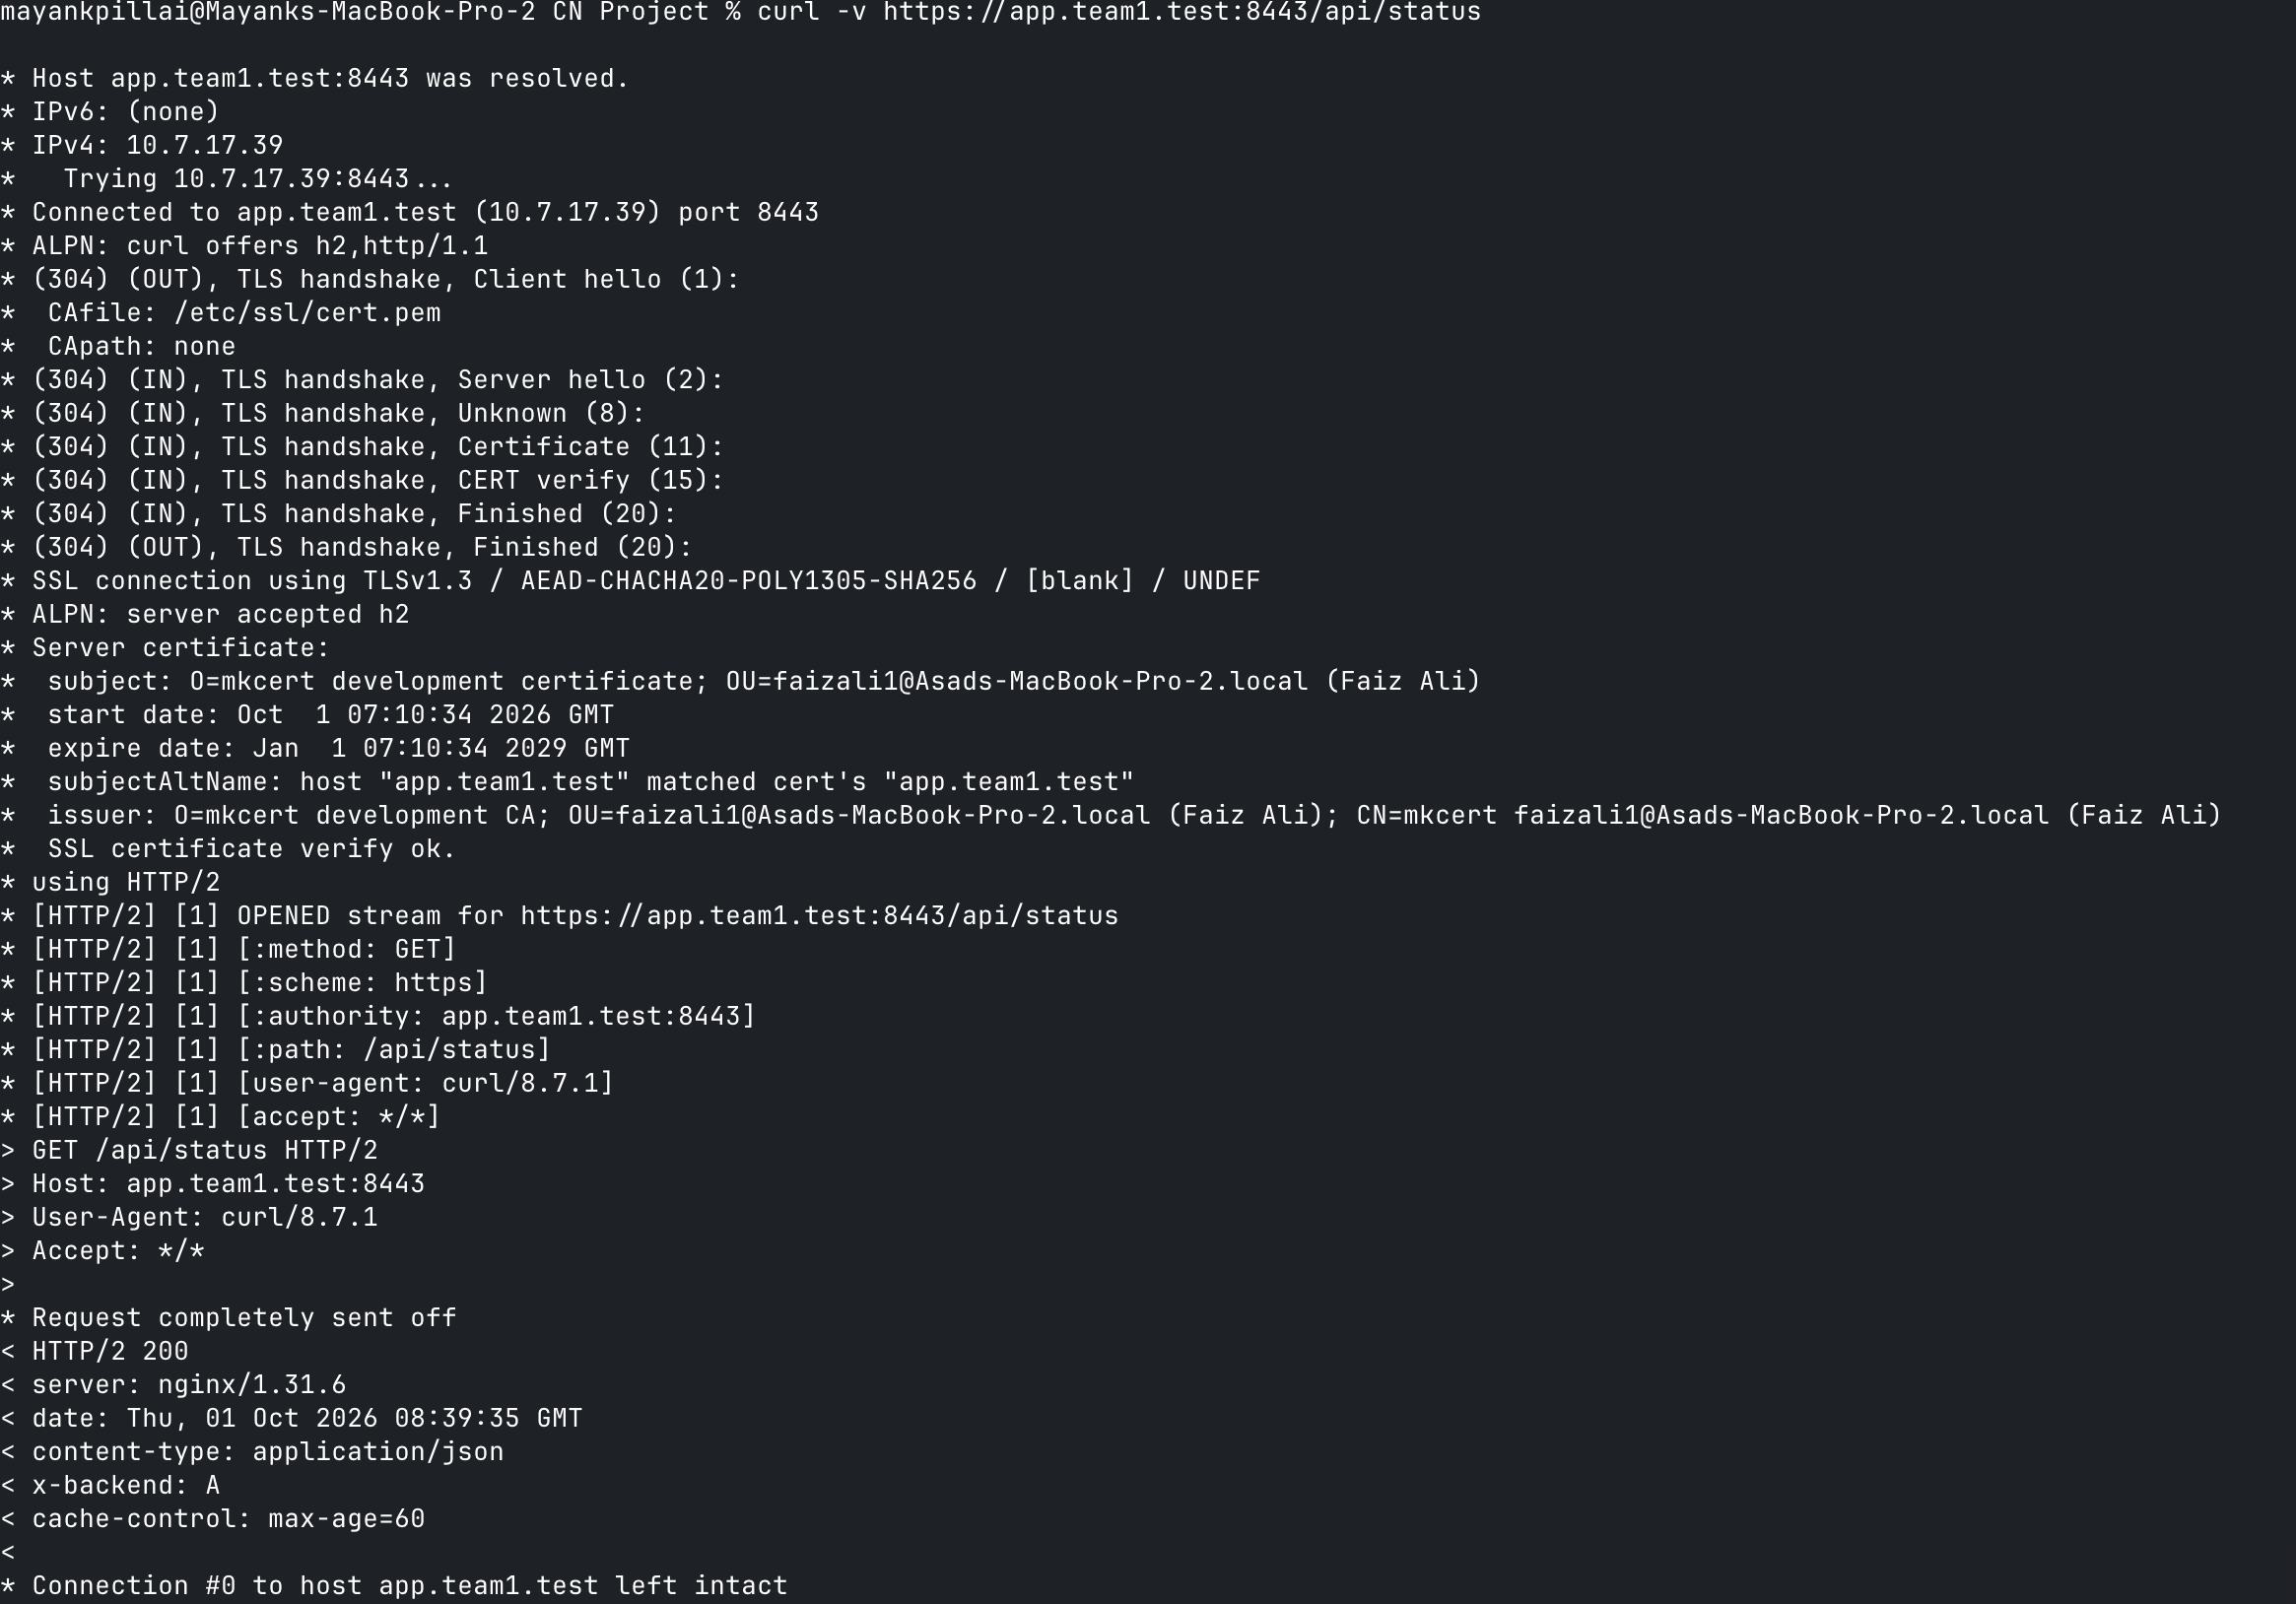
\includegraphics[width=0.9\linewidth]{../evidence/taskE-tls/tls-curl-success-mac3.png}
\caption{Task E: \texttt{curl -v https://app.team1.test:8443/api/status} with no \texttt{-k}.
TLS 1.3, certificate subject name matches \texttt{app.team1.test}, ``SSL certificate verify ok'',
HTTP 200 with \texttt{x-backend: A}.}
\end{figure}

\begin{figure}[H]
\centering
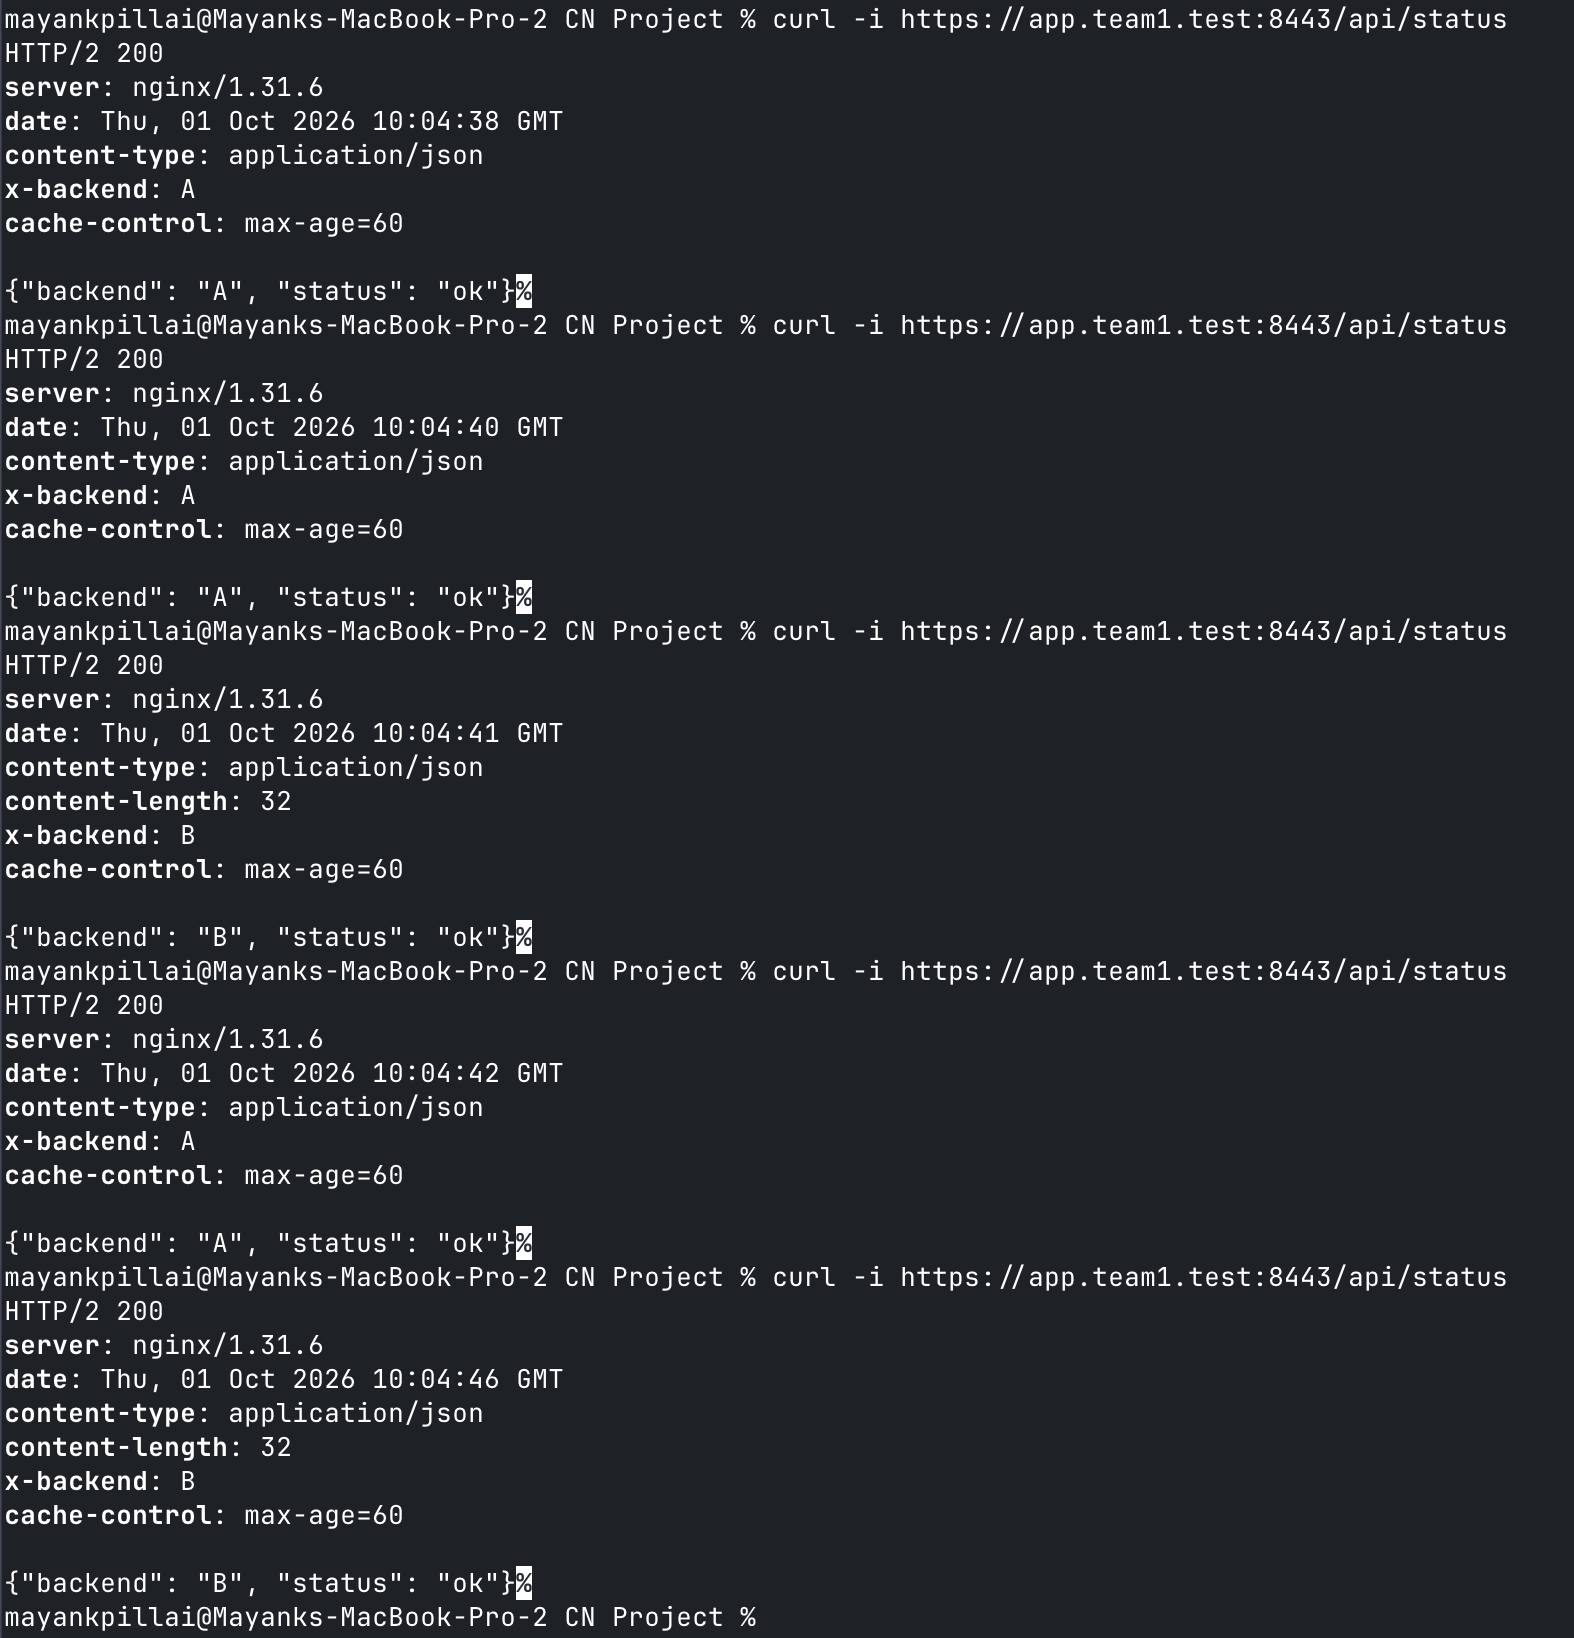
\includegraphics[height=0.42\textheight]{../evidence/taskC-D-load-balancing/load-balancer.png}
\caption{Task D: repeated requests to the same domain are served by both backends
(\texttt{x-backend} A and B).}
\end{figure}

\subsection{HTTP caching (Task F)}
The backends send \texttt{Cache-Control: max-age=60}: a client may reuse the response for 60 seconds
without asking the server again; after that it must fetch it again.
\begin{figure}[H]
\centering
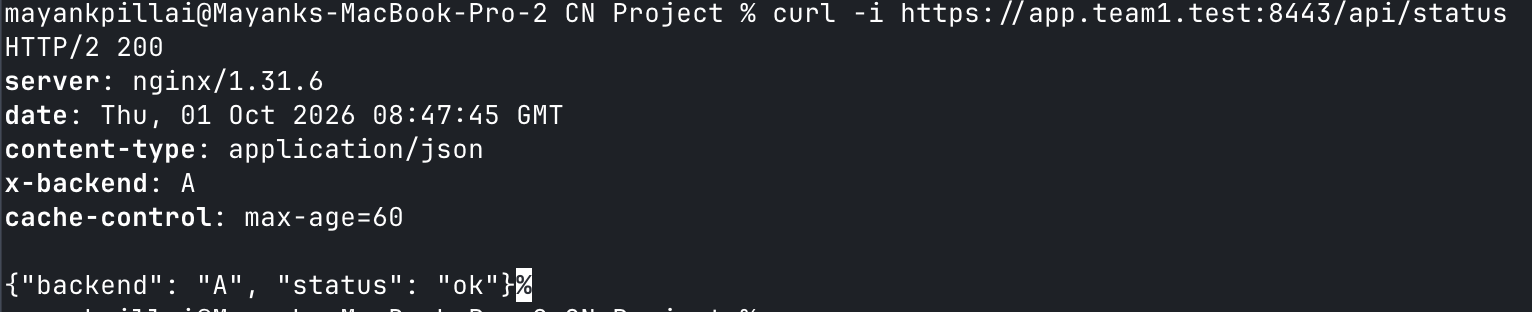
\includegraphics[width=0.85\linewidth]{../evidence/taskF-caching/taskF-curl-headers.png}
\caption{Cache-Control, Date and X-Backend headers in the response.}
\end{figure}

\subsection{Packet evidence (Task G)}
One \texttt{curl} request from Mac 3 (10.7.5.187) to the edge (10.7.17.39), captured in Wireshark.

\textbf{TCP three-way handshake.} The client's port 56982 connects to port 8443: SYN, SYN-ACK, ACK
(frames 3 to 5), before any application data is sent.
\begin{figure}[H]
\centering
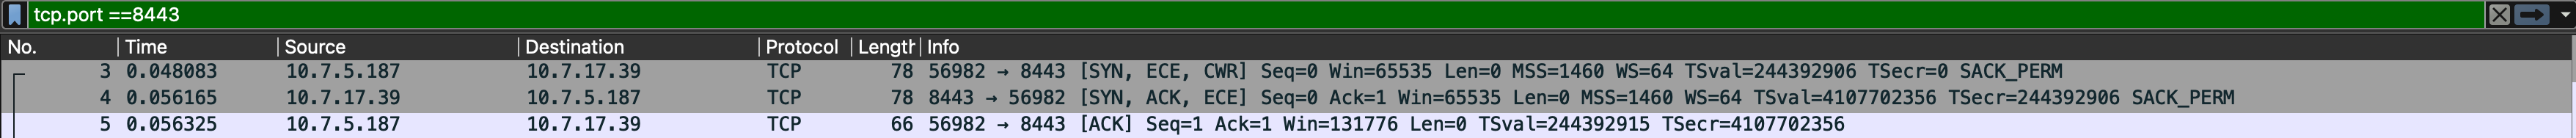
\includegraphics[width=\linewidth]{../evidence/taskG-packet-analysis/tcp-3way.png}
\caption{Filter \texttt{tcp.port==8443}: SYN, SYN-ACK, ACK.}
\end{figure}

\textbf{TLS handshake.} The ClientHello (frame 6, SNI \texttt{app.team1.test}) is answered by the
ServerHello (frame 9), which selects TLS 1.3 with \texttt{TLS\_CHACHA20\_POLY1305\_SHA256}. In TLS 1.3 the
server certificate is encrypted, so it does not appear as a separate packet here; \texttt{curl -v}
(above) shows it.
\begin{figure}[H]
\centering
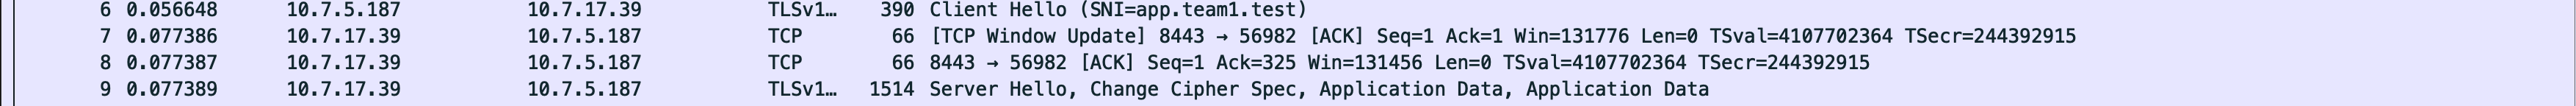
\includegraphics[width=\linewidth]{../evidence/taskG-packet-analysis/TLS-handshake.png}
\caption{ClientHello, then ServerHello with Change Cipher Spec.}
\end{figure}

\textbf{Encrypted payload.} After the handshake every packet is TLS ``Application Data''. The HTTP
headers and body are inside encrypted records, so Wireshark cannot show them; we use \texttt{curl -v}
to show the headers.
\begin{figure}[H]
\centering
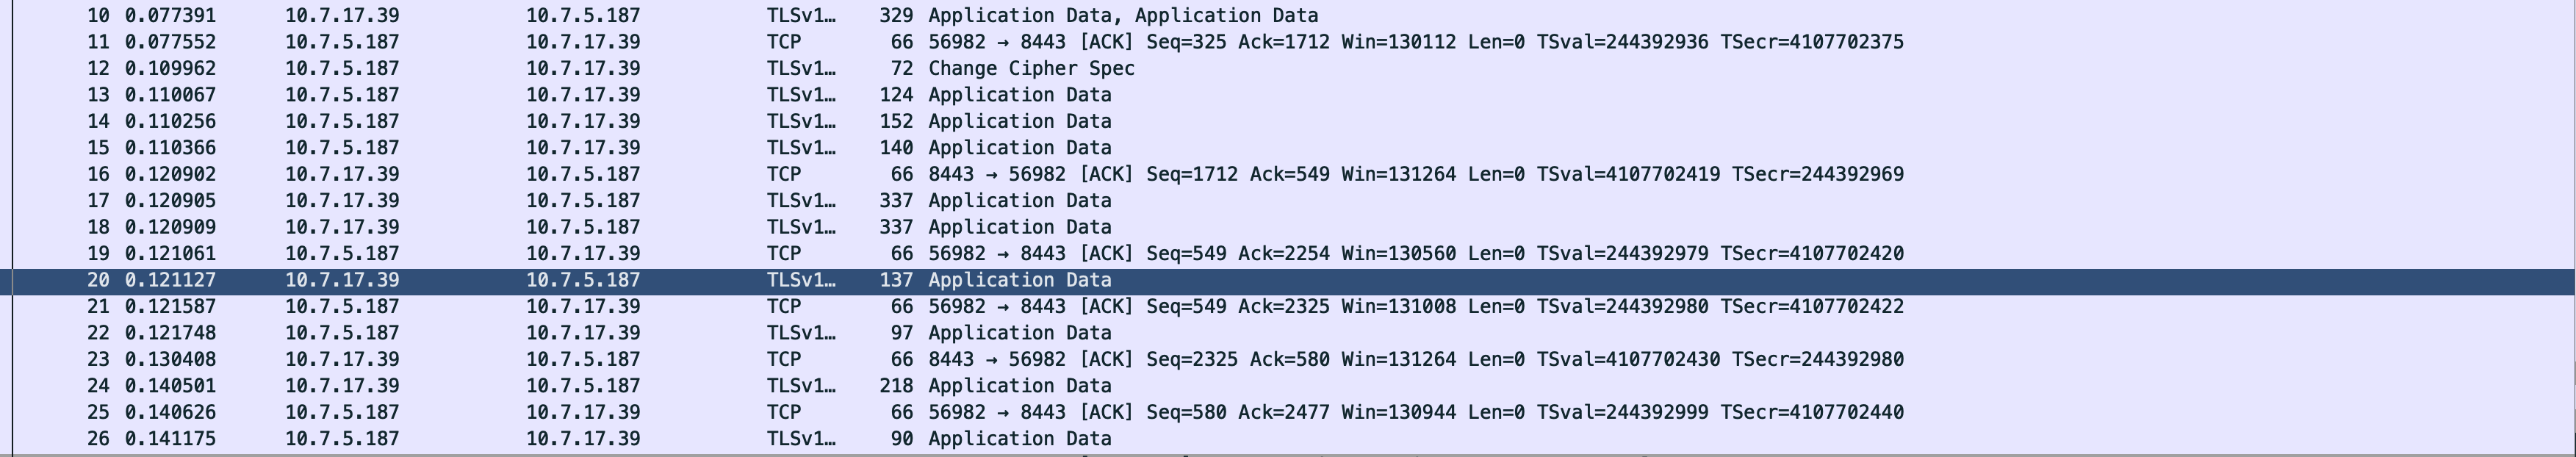
\includegraphics[width=\linewidth]{../evidence/taskG-packet-analysis/application-data.png}
\caption{Only encrypted Application Data after the handshake.}
\end{figure}

% ============================================================
\newpage
\section{Failure Demonstration: Stop One Backend}

\textbf{What we broke:} we stopped Backend A (the Python process on Mac 3, 10.7.5.187:3001).

\textbf{Before:} requests to \texttt{https://app.team1.test:8443/api/status} were served by both
backends (\texttt{x-backend} alternating between A and B; see the load-balancing figure above).

\textbf{After:} every response came from Backend B and still returned HTTP 200.
\begin{figure}[H]
\centering
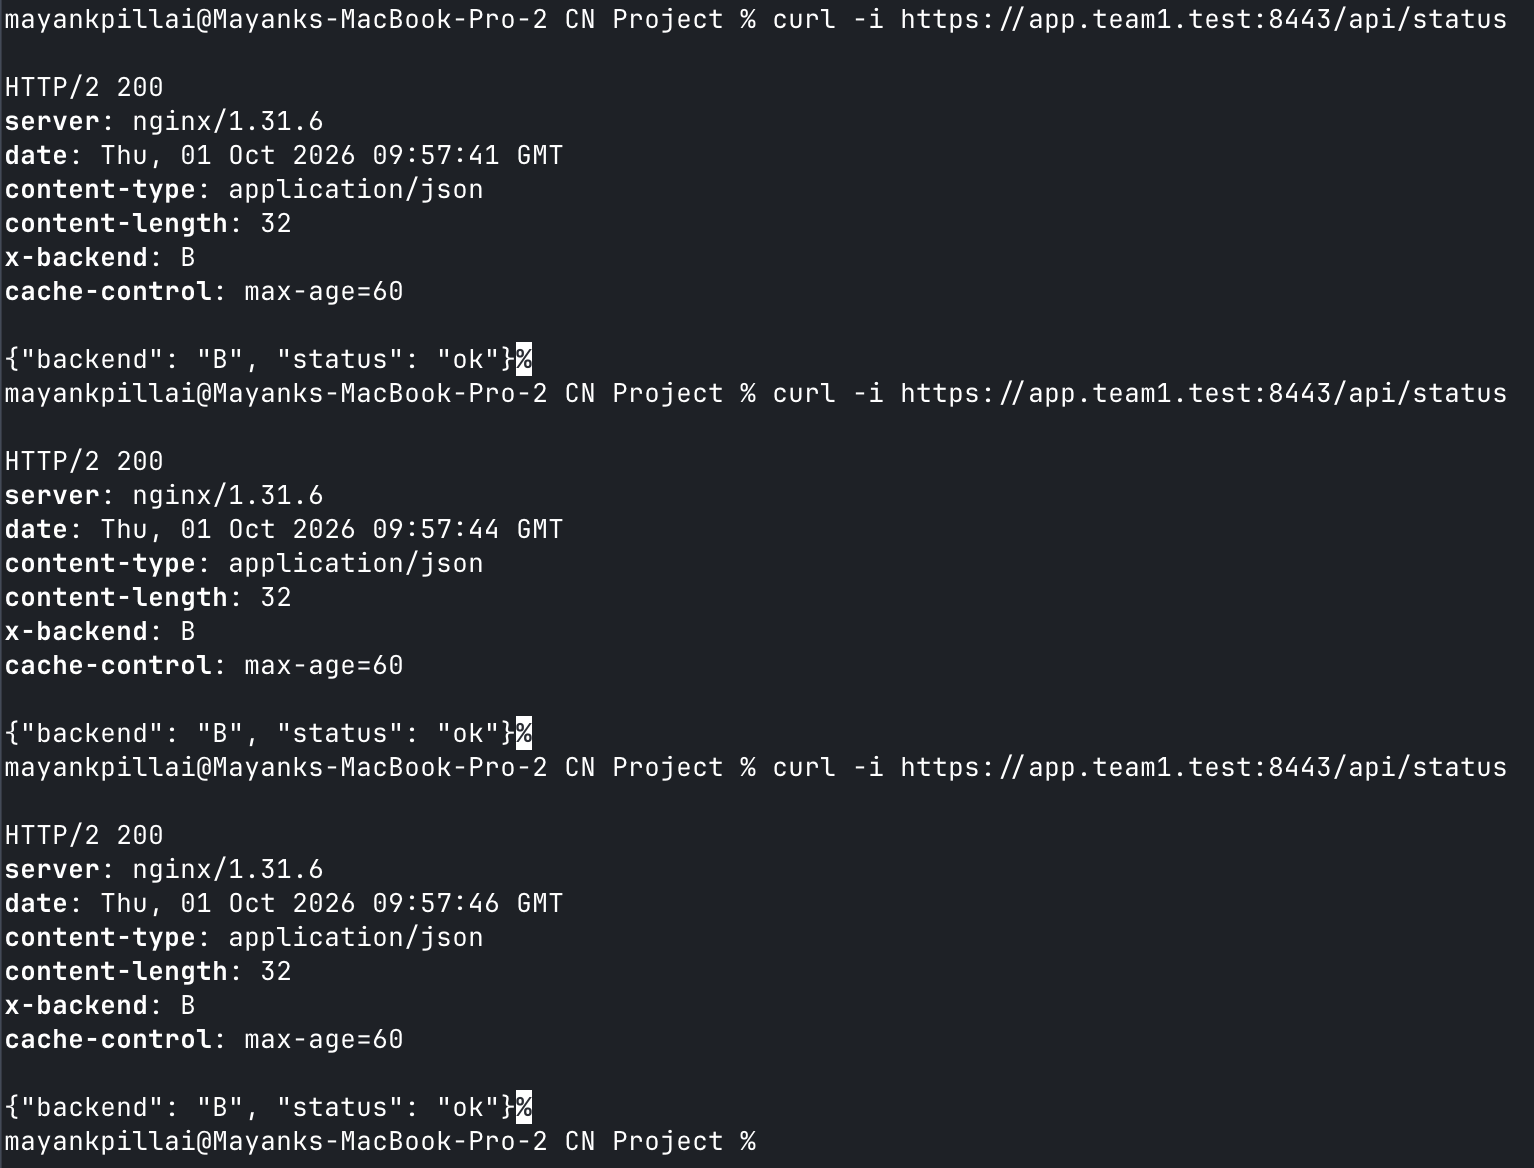
\includegraphics[height=0.38\textheight]{../evidence/failure-scenarios/fail3-one-backend-stopped.png}
\caption{Backend A stopped: three consecutive requests, all \texttt{x-backend: B}, HTTP/2 200.}
\end{figure}

\textbf{Layer affected:} the application / backend service layer behind the load balancer. Port 3001
on Mac 3 stopped accepting connections, so nginx stopped sending requests there and used Backend B.
DNS, IP, the TCP connection to the edge and TLS were not affected: the client still resolved the name,
connected to nginx and completed the TLS handshake. This is why a load balancer gives resilience.

\textbf{Restored:} we restarted Backend A on Mac 3 (\texttt{python3 backend/backend\_a.py}). Afterwards the
same requests were again served by both backends (the load-balancing screenshot was taken after the
failure demonstrations).

\end{document}
